\chapter{Introduction}
%\addcontentsline{toc}{chapter}{Introduction}
......
\section{ATLAS Project}\label{sec:ATLAS}
The ATLAS project was created in 2003 by the Group for Automation and Robotics from the Department of Mechanical Engineering at the University of Aveiro \cite{vsantos2010}. The objective of this project is to study and develop advanced sensors and active systems to promote the autonomous control of cars and other platforms. The first projects in the autonomous driving area focused on small scale models in controlled environments for participation in the National Robotics Festival (FNR) and in many other competitions winning some awards for the best performance (subsection \ref{sec:ATLASplatform}). The success and experience gained with these models allowed the evolution of the project for full-scale vehicles, where ATLASCAR (subsection \ref{sec:ATLASCAR}) in 2010 and ATLASCAR2 (subsection \ref{sec:ATLASCAR2}) in 2016 have been developed.

\subsection{ATLAS platforms}\label{sec:ATLASplatform}	
The first developed robot (Figure \ref{fig:modelosatlas1}) was based on an aluminum and wood structure. In this prototype only one camera was installed that pointed to a mirror to allow the complete visualization of the road in which the robot circulated. The traction movement was assured by a mechanical differential coupled to the rear wheels and the steering movement was given by a single front wheel. In order to create a model more similar to an ordinary car, the ATLAS group developed the ATLAS 2000 (Figure \ref{fig:modelosatlas2}) in scale (1:4), with which it managed to win the first autonomous driving competition of the FNR in 2006. After several improvements made in ATLAS 2000, in 2008 a new platform, ATLAS MV (Figure \ref{fig:modelosatlas3}) was created. This robot was designed on a smaller scale (1:5), with the intention of being lighter and faster. On board were installed a new steering system, hydraulic braking and an active perception unit. This robot allowed the conquest of new victories in the autonomus driving competitions.
\begin{figure}[!h]
	\centering
		\begin{minipage}[t]{0.32\textwidth}
			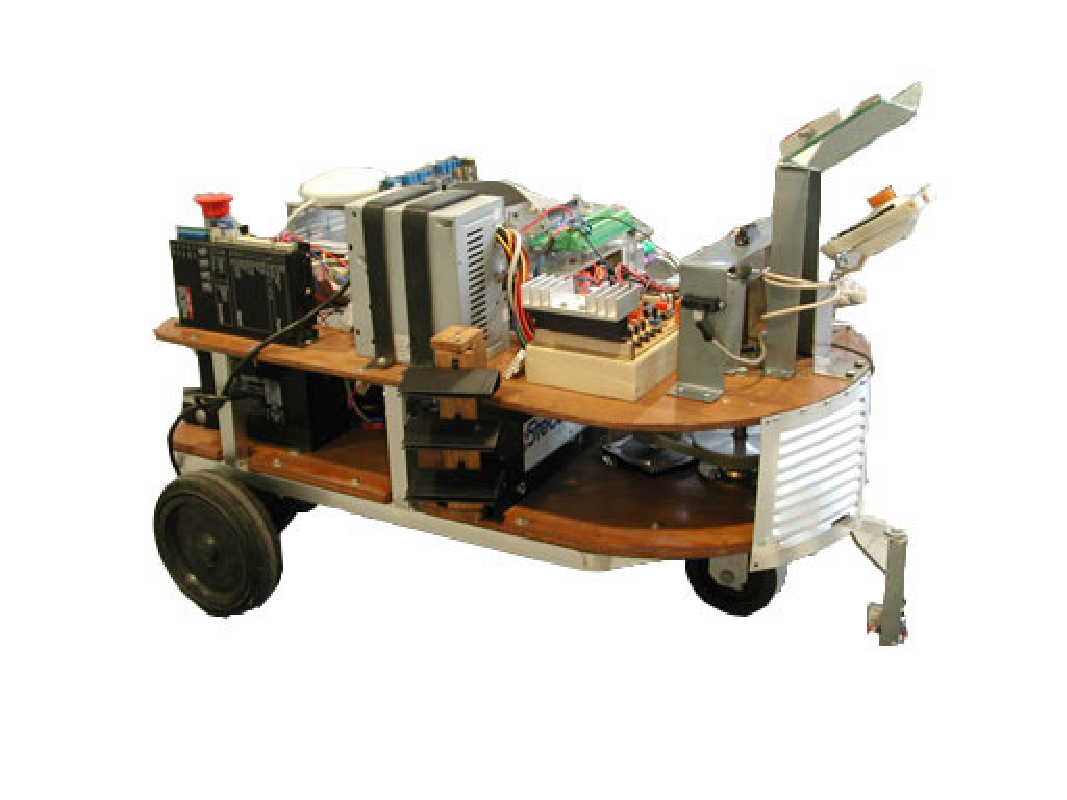
\includegraphics[width=\textwidth]{../figure/modelosatlas1.pdf}
			\subcaption{First ATLAS prototype.}
			\label{fig:modelosatlas1}
		\end{minipage}
		\begin{minipage}[t]{0.32\textwidth}
			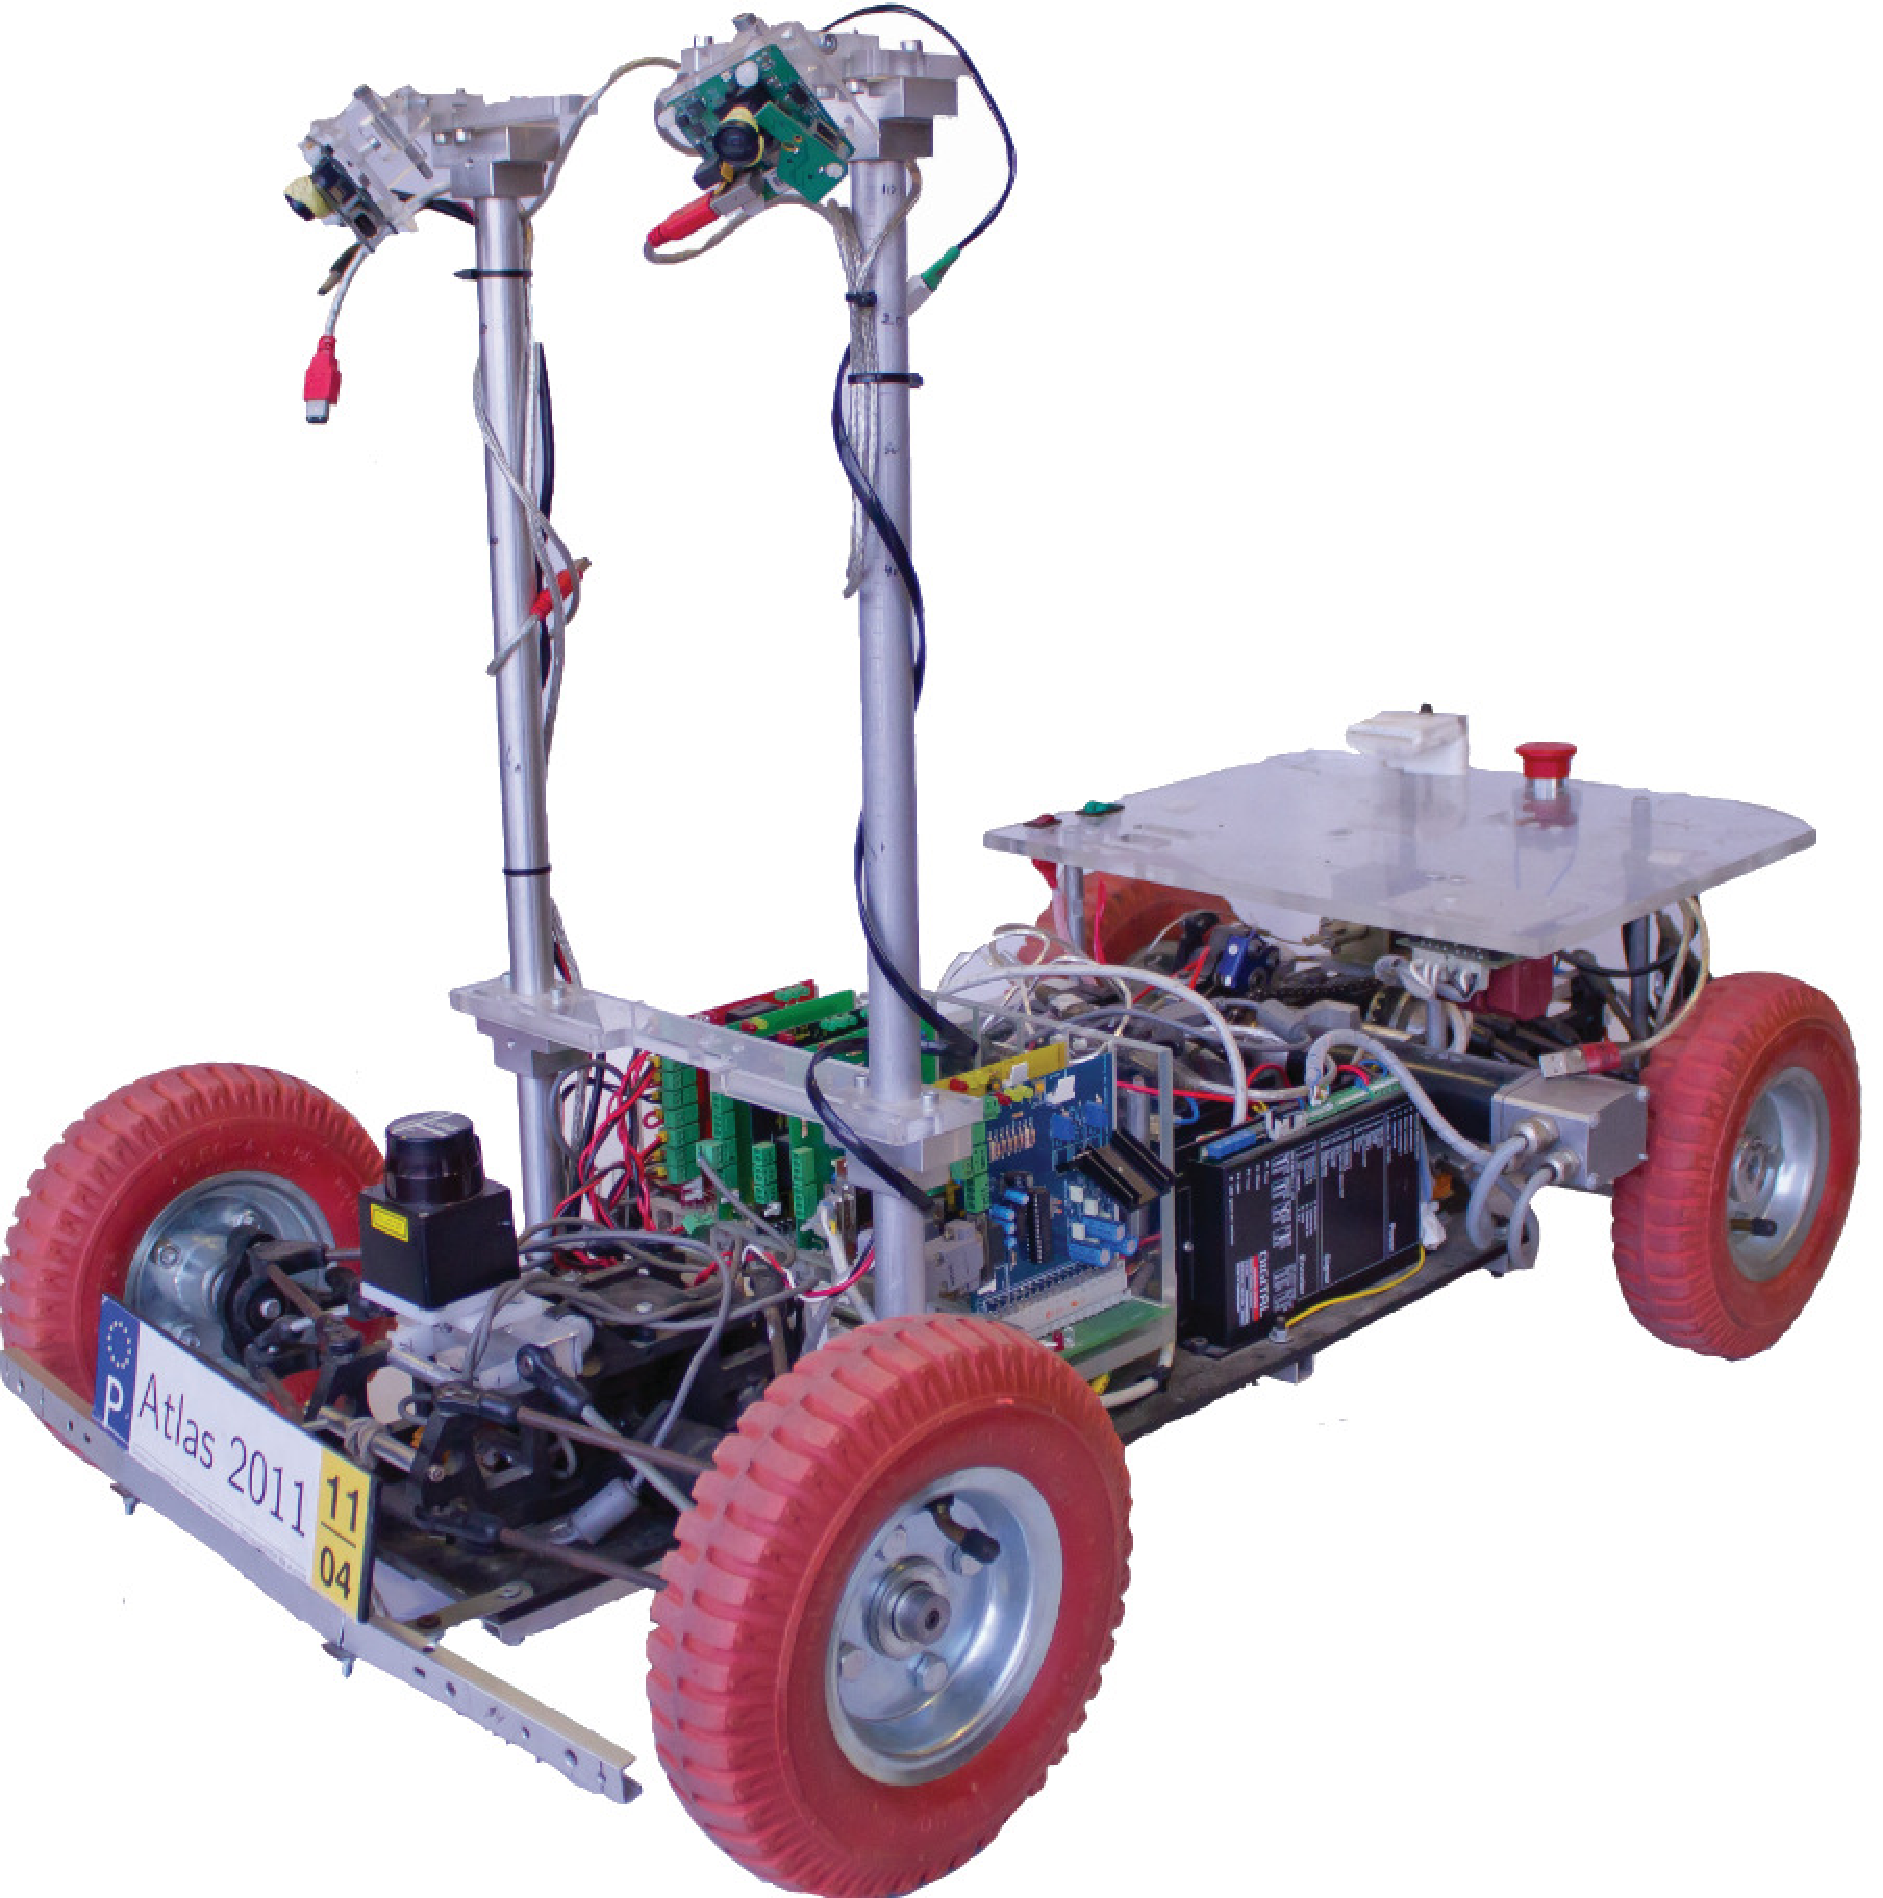
\includegraphics[width=\textwidth]{../figure/modelosatlas2.pdf}
			\subcaption{ATLAS 2000.}
			\label{fig:modelosatlas2}
		\end{minipage}
		\begin{minipage}[t]{0.32\textwidth}
			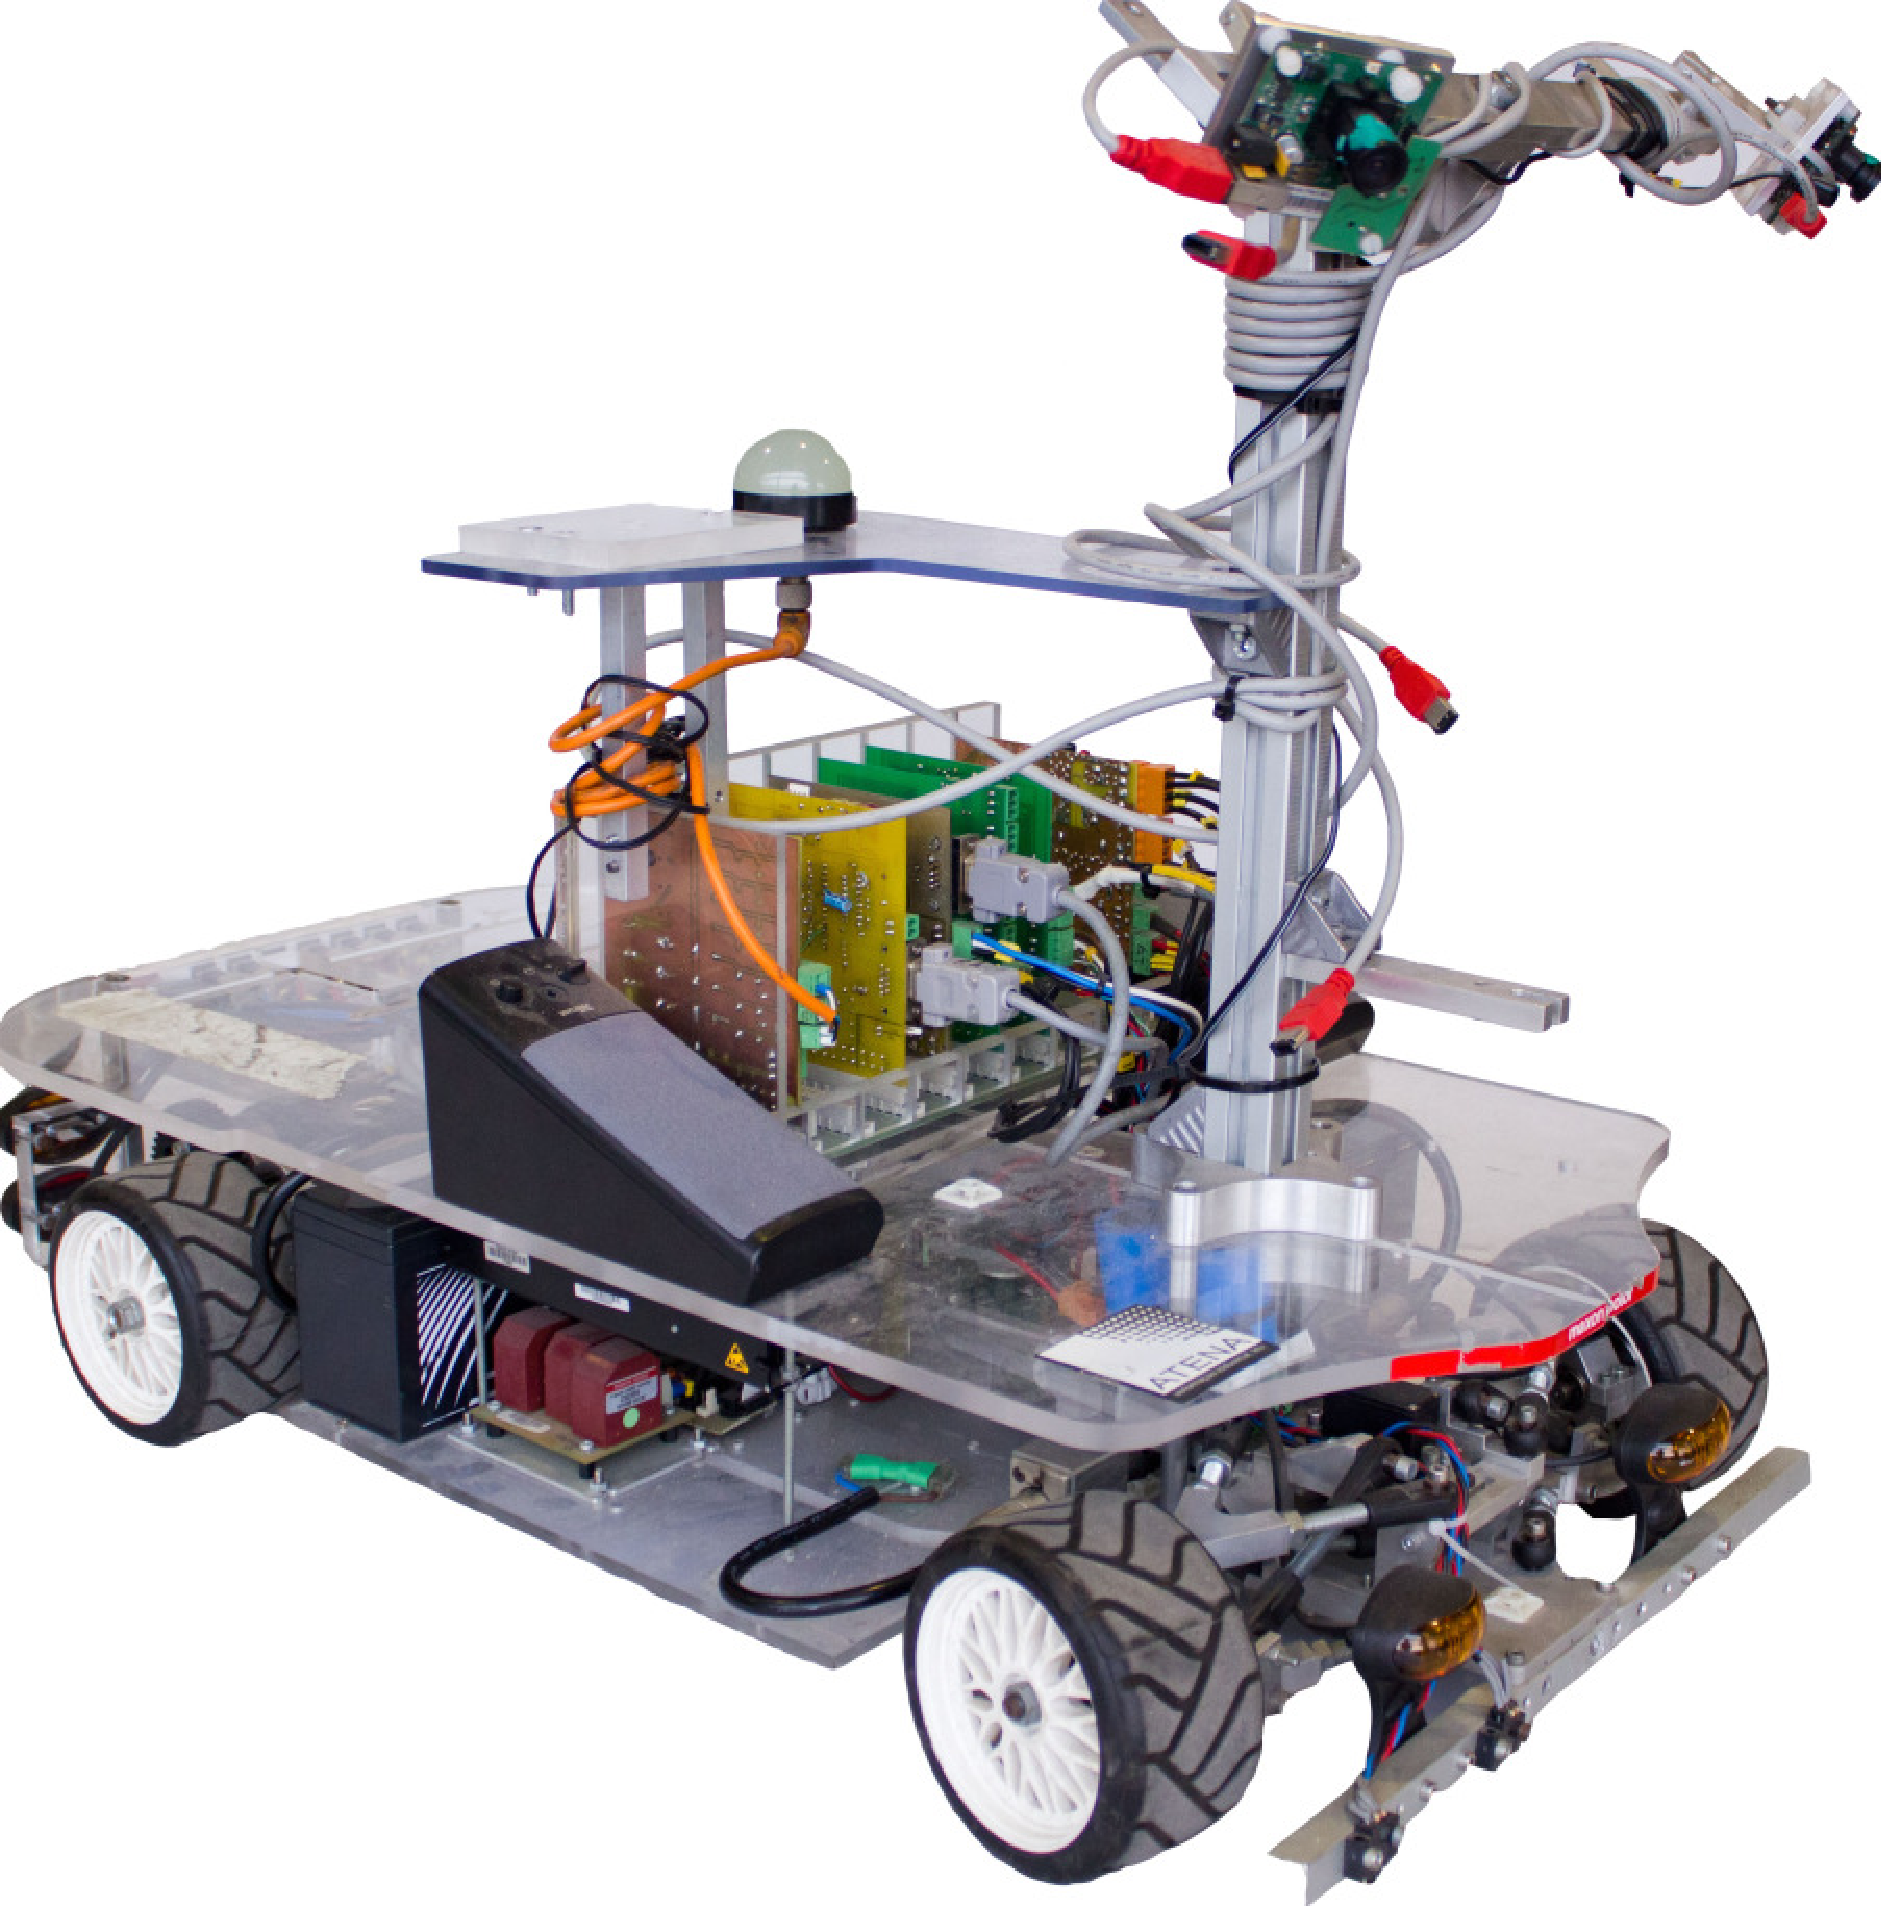
\includegraphics[width=\textwidth]{../figure/modelosatlas3.pdf}
			\subcaption{ATLAS MV.}
			\label{fig:modelosatlas3}
		\end{minipage}
		\caption{Some of the ATLAS project small scale platforms (adapted from \cite{Pereira2012}).}
		\label{fig:modelosatlas}
\end{figure}

\subsection{ATLASCAR}\label{sec:ATLASCAR}
\begin{figure}[!h]
	\centering
	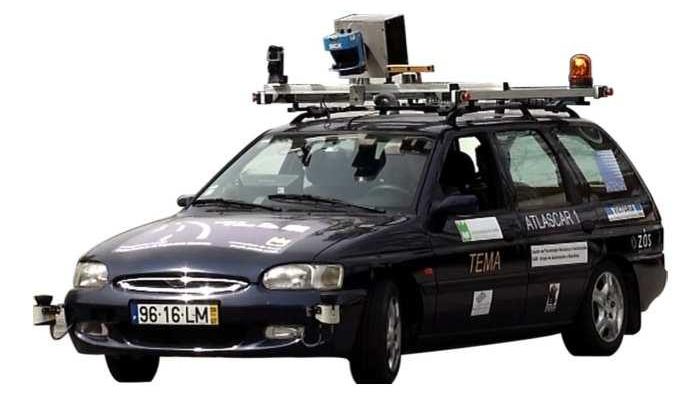
\includegraphics[width=\textwidth]{../figure/atlascar1.jpg}
	\caption{The car used in ATLASCAR, based on Ford Escort Station Wagon of 1998 (adapted from \cite{Pereira2012}).}
	\label{fig:atlascar1}
\end{figure}

\subsection{ATLASCAR2}\label{sec:ATLASCAR2}
\begin{figure}[!h]
	\centering
	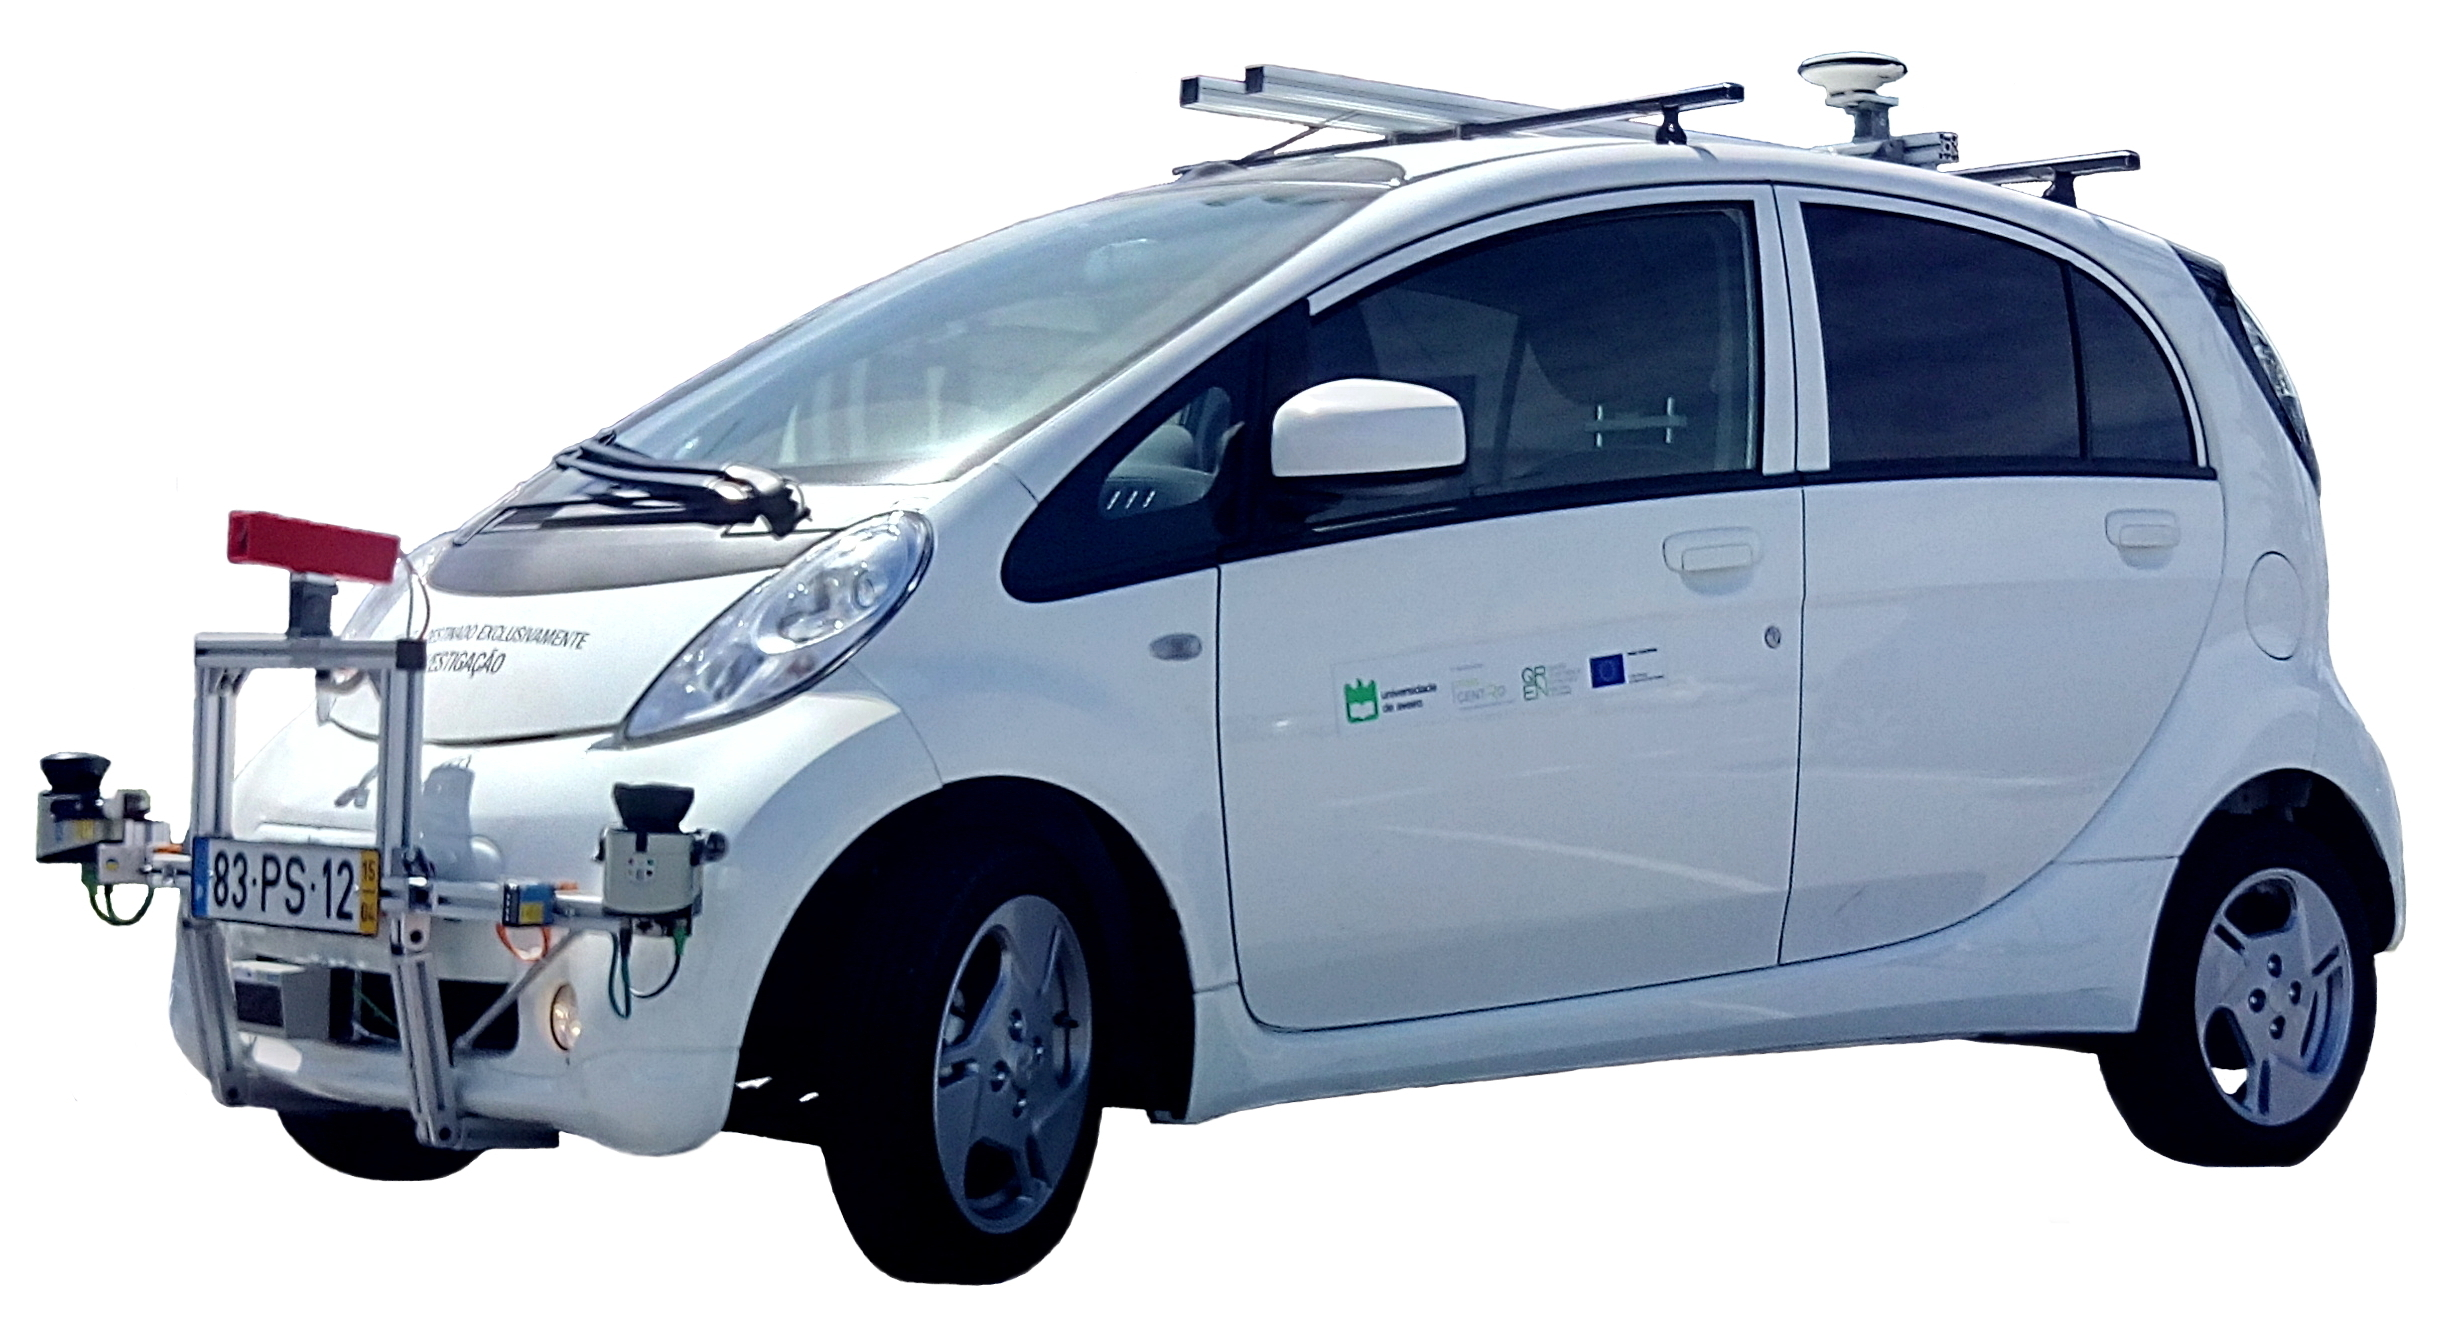
\includegraphics[width=\textwidth]{../figure/atlascar2.jpg}
	\caption{The vehicle used in ATLASCAR2, based on an electric car, a Mitsubishi iMiEV of 2015 (adapted from \cite{Ricardo:Thesis:2018}).}
	\label{fig:atlascar2}
\end{figure}
\section{Context of the Problem and Motivation}
\section{Proposed Approach}
\section{Thesis Outline and Contributions}